% Informe — Pregunta 1, Examen Parcial de Redes Neuronales y Aprendizaje Profundo
%
% Compilar:
%   latexmk -pdf informe.tex
%
% Todas las cifras de este documento provienen de corridas reales del
% repositorio. Lo único pendiente son los nombres del grupo.

\documentclass{article}
\usepackage[preprint]{neurips}

\usepackage[utf8]{inputenc}
\usepackage[T1]{fontenc}
\usepackage[spanish,es-noshorthands]{babel}
\usepackage{amsmath}
\usepackage{url}
\usepackage{multirow}
\usepackage{graphicx}

\title{Clasificación multietiqueta de anomalías de rodilla en resonancia
       magnética con supervisión débil derivada de informes multilingües}

\author{%
  Flavio César Amayo Gamboa \quad \texttt{flavio.amayo.g@uni.pe} \\
  Gustavo Adolfo Huarcaya Delgado \quad \texttt{gustavo.huarcaya.d@uni.pe} \\
  Jhordy Joel Maximiliano Cusi \quad \texttt{jmaximilianoc@uni.pe} \\
  Sergio Mondragon Contreras \quad \texttt{sergio.mondragon.c@uni.pe} \\[0.6em]
  \textbf{Facultad de Ingeniería Industrial y de Sistemas} \\
  Universidad Nacional de Ingeniería
}

\date{31 de octubre de 2026}

% --- Ubicacion de flotantes -------------------------------------------
% Mas margen para que las tablas compartan pagina con el texto en vez de
% irse solas y dejar media pagina en blanco. No cambia margenes ni fuente.
\renewcommand{\topfraction}{0.9}
\renewcommand{\bottomfraction}{0.9}
\renewcommand{\textfraction}{0.07}
\renewcommand{\floatpagefraction}{0.85}
\setcounter{topnumber}{3}
\setcounter{bottomnumber}{2}
\setcounter{totalnumber}{4}

% Titulo de la bibliografia en espanol (neurips.sty lo fija en "References").
\renewcommand{\bibsection}{\section*{\normalsize\bfseries Referencias}}

\begin{document}
\maketitle

\begin{abstract}
Se aborda la predicción simultánea de doce hallazgos clínicos en estudios de
resonancia magnética de rodilla del conjunto RSNA Knee Abnormality Detection,
donde solo 58 de 4\,407 estudios tienen etiquetas verificadas por un radiólogo y
el resto únicamente dispone de su informe en texto libre, redactado en nueve
idiomas. Se construye un pipeline de extracción de etiquetas débiles basado en
reglas con detección de negación y traducción automática selectiva, que alcanza
un 74.3\% de acuerdo contra las etiquetas doradas, con una tasa de ruido estimada
del 25.7\%. Sobre esas etiquetas se entrenan dos arquitecturas 2.5D con
agregación por conjuntos: una red Inception implementada desde cero y una
ResNet-50 preentrenada en ImageNet. ResNet-50 con agregación por promedio, el
modelo del análisis detallado, alcanza un AUC-ROC macro de 0.708 (IC95\%
$[0.662, 0.755]$) sobre los dorados; otra configuración con más datos y atención
por etiqueta llega a 0.761, el mayor valor puntual, con intervalo solapado. Un bootstrap
pareado muestra que solo dos de siete diferencias estudiadas en la ablación son
estadísticamente significativas, y que las dos son decisiones sobre los
\emph{datos} (el preentrenamiento en ImageNet y el plano de la resonancia) y no
sobre la arquitectura. En tres casos, las predicciones más confiadas se apoyan en
regiones anatómicamente plausibles; solo 3 de 12 hallazgos muestran activación
consistente. La evaluación por idioma documenta un sesgo lingüístico marcado que
persiste tras la mitigación.
\end{abstract}

% ============================================================================
\section{Motivación}
% ============================================================================

La resonancia magnética es el estudio de referencia para evaluar lesiones de
ligamentos, meniscos y cartílago de la rodilla, pero su interpretación depende de
radiólogos musculoesqueléticos y está sujeta a variabilidad inter-observador.
Fuera de los grandes centros la demora entre el estudio y su informe se mide en
semanas, y un clasificador automático podría priorizar estudios o actuar como
segunda lectura.

La dificultad no es la que suele plantearse en los conjuntos curados de visión
por computadora. En este problema, la supervisión disponible es el obstáculo
principal: de 4\,407 estudios de entrenamiento, solo 58 cuentan con las doce
etiquetas verificadas por un radiólogo. Los 4\,349 restantes aportan únicamente
el informe original en texto libre, redactado en uno de nueve idiomas por
profesionales de 16 centros en cinco continentes.

Esa asimetría desplaza el trabajo hacia una pregunta que rara vez se formula:
antes de entrenar cualquier red hay que construir las etiquetas y cuantificar
cuán sucias quedaron. Este informe sostiene que esa cuantificación (y no la
elección de arquitectura) es lo que gobierna el resultado final.

% ============================================================================
\section{Trabajos relacionados}
% ============================================================================

\paragraph{Arquitecturas convolucionales.}
La progresión de LeNet~\citep{lecun1998gradient} a
AlexNet~\citep{krizhevsky2012imagenet} y VGG~\citep{simonyan2015very}
estableció que apilar convoluciones con reducciones sucesivas de resolución
produce representaciones jerárquicas útiles, al costo de un crecimiento rápido
en parámetros. Inception~\citep{szegedy2015going} aborda ese costo con ramas
paralelas de distinto tamaño de núcleo; las redes
residuales~\citep{he2016deep} atacan otro problema (la degradación del
entrenamiento con la profundidad) mediante conexiones de salto. El
preentrenamiento sobre ImageNet~\citep{deng2009imagenet} es la práctica
habitual con conjuntos de destino pequeños, y acá resulta una de las dos
únicas decisiones significativas (Sección~\ref{sec:ablacion}).

\paragraph{Agregación de instancias.}
La predicción es por estudio, pero la red observa cortes. El marco de aprendizaje
de múltiples instancias con atención~\citep{ilse2018attention} formula esa
agregación como una suma ponderada cuyos pesos la red aprende, con una compuerta
multiplicativa que suprime instancias irrelevantes. Este trabajo sigue esa
formulación; la ablación muestra que, con 416 estudios de entrenamiento, un
promedio sin parámetros queda por delante sin que la diferencia alcance
significancia.

\paragraph{Interpretabilidad y desbalance.}
Grad-CAM~\citep{selvaraju2017grad} produce mapas de localización a partir del
gradiente de una salida respecto del último mapa convolucional, sin modificar la
arquitectura ni reentrenar; se emplea aquí para juzgar si las regiones en que se
apoya el modelo son anatómicamente plausibles. Para el desbalance, la pérdida
focal~\citep{lin2017focal} reescala cada término por $(1-p_t)^\gamma$ para
reducir la contribución de los ejemplos ya resueltos, y se evalúa junto con una
ponderación por prevalencia inversa.

\paragraph{Extracción de información desde texto clínico.}
NegEx~\citep{chapman2001simple} resuelve el problema central de leer informes
médicos: distinguir un hallazgo afirmado de uno explícitamente descartado,
mediante disparadores léxicos dentro de una ventana alrededor del término. La
Sección~\ref{sec:etiquetas_resultados} cuantifica cuánto cambia el resultado al
incorporarlo. Para los informes en idiomas que el extractor no lee de forma
nativa se emplea NLLB-200~\citep{nllb2022}.

% ==========================================================================
\section{Conjunto de datos}
% ============================================================================

El conjunto RSNA Knee Abnormality Detection~\citep{rsna2026knee} contiene
819\,640 archivos DICOM (569.76~GB) correspondientes a 4\,407 estudios de
entrenamiento. Cada estudio incluye entre 3 y 14 series, con una mediana de 28
cortes por serie.

El enunciado menciona aproximadamente doce idiomas; la detección automática sobre
los informes arroja nueve lenguas: inglés (39.4\%), español (15.5\%), turco
(12.4\%), croata (9.2\%), griego (7.3\%), alemán (5.9\%), búlgaro (5.0\%),
neerlandés (3.5\%) y francés (1.8\%). Dos de ellas no emplean alfabeto latino.

La heterogeneidad técnica de las imágenes es considerable. Sobre una muestra de
764 cortes se midieron diez resoluciones distintas entre $320\times320$ y
$1024\times1024$, espaciados de píxel entre 0.146 y 0.562~mm (un factor de
cuatro), campos de visión físicos de 130 a 240~mm, ocho fabricantes,
intensidades de campo de 1.5~T y 3~T, y profundidades de 12 y 16 bits. La
etiqueta \texttt{Laterality} está ausente o vacía en el 54\% de los cortes, y el
campo \texttt{SeriesDescription} resulta inutilizable como filtro: presenta 21
valores distintos, incluido el literal \texttt{DummySeriesDesc!} en el 10\% de los
casos.

% ============================================================================
\section{Metodología}
% ============================================================================

\subsection{Extracción de etiquetas débiles}

El extractor procesa cada informe oración por oración, en lugar de sobre el texto
completo: operar sobre el informe entero permitiría que un término patológico de
una oración se asociara con una estructura anatómica mencionada en otra.

Siete de las doce etiquetas exigen la coincidencia simultánea de un término
anatómico y uno patológico dentro de la misma oración. Mencionar el ligamento
cruzado anterior no constituye un hallazgo: prácticamente todos los informes lo
nombran, habitualmente para declararlo íntegro. Las cinco restantes (derrame
articular, sinovitis, quiste de Baker, contusión ósea y fractura) son hallazgos
directos cuyo término ya denota la patología.

Sobre cada coincidencia se aplica un clasificador de aserción siguiendo el
esquema NegEx~\citep{chapman2001simple}: una ventana de seis palabras alrededor
del término se examina en busca de disparadores previos (\emph{no},
\emph{without}, \emph{sin}) y posteriores (\emph{is intact}, \emph{not torn},
\emph{conservado}), más un conjunto de expresiones de incertidumbre.

Los informes en los siete idiomas que el extractor no lee de forma nativa se
traducen al inglés con NLLB-200-distilled-600M~\citep{nllb2022}, oración por
oración. La traducción por oraciones es necesaria porque los informes alcanzan
4\,743 caracteres, más de lo que el modelo procesa en una pasada, y además
preserva la estructura sobre la que opera el extractor.

Extender el diccionario de términos a los siete idiomas restantes no habría
resuelto el problema. El detector de negación opera sobre palabras separadas
dentro de una ventana, y el turco niega mediante un sufijo
(\emph{yırtılmamış}, ``no desgarrado''), mientras que el griego y el búlgaro
añaden un alfabeto distinto. Traducir el texto completo convierte nueve problemas
de negación en el único que ya está resuelto y medido.

\subsection{Preprocesamiento}

Dada la dispersión de espaciados de píxel documentada en la Sección~3,
redimensionar directamente a $224\times224$ entregaría la misma estructura
anatómica a escalas físicas dispares: la red debería aprender configuraciones de
escáner antes de poder aprender anatomía.

El pipeline recorta en consecuencia una ventana de 130~mm \emph{físicos},
empleando el espaciado de píxel del encabezado DICOM, y redimensiona después. La
intensidad se normaliza por corte entre sus percentiles 1 y 99, dado que la
resonancia magnética carece de unidades absolutas: el mismo tejido registra 636
en un escáner y 2\,781 en otro. La lateralidad se resuelve con la etiqueta
\texttt{Laterality} cuando está presente y, en su defecto, mediante el signo de la
coordenada $x$ del sistema de coordenadas del paciente; cuando ninguna fuente
responde, la serie se deja sin modificar antes que invertirla por conjetura.

De cada serie se descarta el 20\% de cortes en cada extremo (mayormente aire y
diáfisis) y de la banda central se extraen ocho grupos de tres cortes
contiguos, uniformemente espaciados. La elección de tres canales es deliberada:
los pesos de ImageNet esperan exactamente tres, de modo que la primera
convolución preentrenada se carga sin modificación alguna.

No se emplea procesamiento volumétrico 3D. El espaciado entre cortes (2.875~mm)
supera entre 6 y 20 veces al espaciado dentro del corte, de modo que el volumen
es marcadamente anisotrópico: un núcleo $3\times3\times3$ mezclaría 1.5~mm en el
plano con 8.6~mm entre cortes.

\subsection{Selección del subconjunto}

Se trabaja con 576 estudios, dentro del rango recomendado. Un muestreo aleatorio
no sería adecuado: con 182 positivos de fractura entre 4\,407 estudios, una
extracción aleatoria de 600 contendría unos 25, insuficientes tanto para aprender
como para medir.

El muestreo procede en tres pasadas. Primero se incorporan todos los estudios
dorados, que constituyen el conjunto de prueba. Luego se completan cuotas por
etiqueta, recorriéndolas de la más rara a la más frecuente; el orden importa,
porque un estudio positivo en fractura suele serlo también en algún hallazgo
común, de modo que las etiquetas frecuentes se completan solas mientras que las
raras nunca lo harían. El resto se extrae al azar, para que la muestra represente
la distribución real y no exclusivamente patología. La muestra resultante
garantiza al menos 73 positivos por etiqueta.

Se excluyen los estudios en que el extractor no halló evidencia alguna. No se
trata de rodillas sanas, sino de informes que el extractor no pudo leer;
entrenar con ellos equivaldría a enseñarle al modelo que estudios con patología
real son completamente negativos.

\subsection{Arquitecturas}

Ambos modelos comparten toda la cadena excepto el codificador:

\begin{equation*}
(B, 8, 3, 224, 224)
\;\xrightarrow{\ \text{codificador}\ }\; (B, 8, D)
\;\xrightarrow{\ \text{agregación}\ }\; (B, D)
\;\xrightarrow{\ \text{cabeza}\ }\; 12 \text{ logits}
\end{equation*}

El \textbf{modelo A} emplea un codificador Inception escrito desde cero, con
cuatro bloques y 0.58~M parámetros en el codificador (0.7~M en el modelo
completo). Se eligió Inception sobre una pila residual por una razón vinculada al
dominio: sus ramas paralelas observan campos receptivos de $1\times1$, $3\times3$
y $5\times5$ a la misma profundidad, y los hallazgos de rodilla se manifiestan a
escalas muy dispares: una rotura meniscal abarca milímetros, un derrame ocupa
la cápsula articular. Con 576 estudios, capturar ambas escalas sin profundizar
resulta más valioso que la profundidad en sí.

El \textbf{modelo B} emplea ResNet-50 con pesos de ImageNet (24.1~M parámetros),
descartando su cabeza de clasificación y conservando la característica agrupada
de 2\,048 dimensiones.

La agregación y la cabeza multietiqueta son idénticas en ambos. La agregación por
atención sigue la formulación con compuerta de~\citet{ilse2018attention}: una red
pequeña puntúa cada grupo, los puntajes se normalizan con softmax y el embedding
del estudio es su suma ponderada. Un promedio diluiría el hallazgo (una rotura
meniscal abarca dos o tres cortes de treinta) y un máximo descartaría la
evidencia corroborante.

\subsection{Atención por etiqueta y reparto por plano}
\label{sec:por-caras}

Una atención compartida obliga a las doce etiquetas a ponderar los cortes de la
misma manera, y los hallazgos no viven en los mismos: un derrame ocupa la
cápsula, una rotura meniscal dos o tres cortes centrales. Las configuraciones
C--E usan doce atenciones. El codificador y la proyección siguen compartidos
(hasta ahí nada depende de qué se busca) y la separación ocurre en la
compuerta, de modo que cada etiqueta elige sus grupos sin multiplicar el costo
del codificador.

Estas configuraciones se entrenan sobre los 4\,407 estudios, no sobre los 576:
de cada estudio se extraen 64 grupos en vez de 8, la partición reserva los 56
dorados como prueba y divide el resto en 80\% de entrenamiento y 20\% de
validación, y el preprocesamiento es el mismo salvo el plano, que deja de ser
únicamente sagital.

El reparto por plano responde a que una estructura se ve o no según la dirección
del corte. La artrosis patelofemoral es el desgaste entre la rótula y el surco
femoral: el corte axial muestra esa superficie completa y el coronal la superpone
al fémur, y medido sobre validación la etiqueta gana 0.060 de AUC al cambiar de
plano ---el mayor efecto por etiqueta al cambiar de plano. El menisco lateral
pierde 0.033, coherente con ser una estructura horizontal que el axial corta en
su propio plano. La configuración D entrena un modelo Inception por cada uno de
los tres planos (sagital, axial y coronal) y rutea cada etiqueta al plano donde
rinde mejor en validación; la E añade una cuarta corrida ResNet-50 para las dos
etiquetas (menisco lateral y artrosis patelofemoral) que mejoran al cambiar de
plano, de ahí que D tenga tres modelos y E cuatro. El reparto se decidió sobre
validación; los dorados se usaron una sola vez, ya fijado.

\subsection{Protocolo de evaluación}

Las decisiones de arquitectura, función de pérdida, agregación, número de épocas
y umbral se toman exclusivamente mediante validación sobre las etiquetas débiles
(416 estudios de entrenamiento, 104 de validación). El umbral es único por
configuración ---no uno por etiqueta---: se elige en validación el valor que
maximiza el $F_1$ macro y se aplica sin modificación sobre los dorados. De los 58
estudios con etiqueta de radiólogo, 2 no aportan una serie sagital sensible a
líquido con supresión grasa y quedan fuera del subconjunto preprocesado, de modo
que la prueba se realiza sobre los 56 restantes, una única vez, al final, para la
cifra que se reporta. El enunciado sugiere reservarlos como validación limpia;
usarlos como prueba final es más estricto, porque evita seleccionar modelos sobre
56 estudios.

Con 56 estudios de prueba y nueve positivos
de ligamento colateral medial, seleccionar el modelo contra ese conjunto no
mediría generalización sino el grado de sobreajuste de la propia selección, y la
cifra posterior se informaría sobre los mismos datos empleados para elegir. La
regla se mantiene por su propio fundamento, con independencia de cualquier
observación empírica puntual.

Todo intervalo de confianza se obtiene por bootstrap sobre 2\,000 remuestreos.
Las comparaciones entre configuraciones emplean bootstrap \emph{pareado}: ambos
modelos se evalúan sobre los mismos estudios, de modo que sus errores están
correlacionados y comparar intervalos independientes resultaría excesivamente
conservador.

% ============================================================================
\section{Experimentos y resultados}
% ============================================================================

\subsection{Extracción de etiquetas débiles}
\label{sec:etiquetas_resultados}

Un buscador de términos sin tratamiento de negación alcanza apenas un 48.3\% de
acuerdo en derrame articular y produce 112 falsos positivos sobre 58 estudios. La detección de negación elimina 29 de esos 112 falsos positivos sin perder un verdadero positivo. La causa es estructural: los informes radiológicos
enumeran tanto lo que el radiólogo encontró como lo que descartó
(\emph{``ACL is intact''}, \emph{``no fracture is seen''}, \emph{``medial
meniscus is not torn''}), de modo que un buscador de términos marca positivo
precisamente donde el informe declara la estructura sana.

Se compararon cuatro estrategias de traducción sobre los mismos 58
dorados. Sin traducir, el acuerdo macro es 72.1\% ($F_1$ 0.512, ruido 27.9\%);
traducir todo lo lleva a 74.0\% ($F_1$ 0.556, ruido 26.0\%); y el esquema híbrido
(traducir salvo inglés y español) a 74.3\% ($F_1$ 0.589), con la tasa de ruido en
25.7\%. Los modelos se entrenaron con las etiquetas de este híbrido, de modo que
25.7\% es el ruido de entrenamiento y 26.0\% una medición del estudio de
traducción. Traducir todo y traducir salvo inglés dan el
mismo resultado hasta la tercera cifra: traducir inglés a inglés no cambia nada
medible, y la mejora proviene solo de \emph{no} traducir el español.

La mejora del esquema híbrido sobre la línea base es de $+0.076$ en $F_1$ macro,
con IC95\% $[+0.039, +0.127]$ por bootstrap pareado sobre estudios: el intervalo
de la diferencia no cruza cero, aunque los sueltos se solapen.

El español se tradujo deliberadamente como experimento de control. Puesto que el
extractor lo lee de forma nativa con $F_1$ 0.48, una traducción que no degradara
información debería arrojar un valor comparable. El resultado observado es 0.29,
una caída de 19 puntos que confirma que el traductor deteriora la terminología
médica y justifica excluir el español del esquema final. El inglés, que no se
traduce, permanece en 0.66 y verifica que el pipeline no altera lo que no debe.

\begin{table}[htbp]
\centering
\caption{$F_1$ macro por idioma sobre los estudios dorados, antes y después de la
         traducción, y proporción de estudios sin ninguna etiqueta positiva sobre
         el conjunto completo.}
\begin{tabular}{lccccc}
\toprule
\multirow{2}{*}{Idioma} & \multirow{2}{*}{$n$ dorados} &
\multicolumn{2}{c}{$F_1$ macro} & \multicolumn{2}{c}{Sin etiqueta} \\
\cmidrule(lr){3-4}\cmidrule(lr){5-6}
 & & Antes & Después & Antes & Después \\
\midrule
Inglés     & 28 & 0.66 & 0.66 & 11.5\% & 11.5\% \\
Español    & 10 & 0.48 & 0.29 & 18.9\% & 18.9\% \\
Turco      &  6 & 0.04 & 0.34 & 87.5\% & 25.1\% \\
Croata     &  4 & 0.00 & 0.21 & 93.1\% &  9.4\% \\
Griego     &  3 & 0.00 & 0.11 & 90.3\% & 54.2\% \\
Búlgaro    &  3 & 0.00 & 0.32 & 99.5\% & 10.9\% \\
Neerlandés &  2 & 0.06 & 0.44 & 94.8\% & 17.6\% \\
Alemán     &  2 & 0.08 & 0.19 & 63.7\% & 26.7\% \\
\bottomrule
\end{tabular}
\end{table}

La proporción global de estudios sin ninguna etiqueta positiva desciende del
46.8\% al 18.3\% (807 de 4\,407).

El extractor subdetecta, pero no de forma uniforme, y la diferencia
importa. El cociente entre la prevalencia extraída sobre los 4\,407 estudios y
la observada en los dorados va de 1.02 en menisco medial (45.6\%
frente a 44.8\%, no subdetecta nada) a 0.22 en sinovitis. Las tres
peores no fallan por el mismo motivo: sinovitis es la única donde el recall
medido también se hunde (0.37), mientras que fractura tiene recall 0.78 y
extrae poco simplemente porque es poco prevalente. Esa distinción separa la
etiqueta ruidosa de la rara, dos problemas con soluciones distintas.

\subsection{Curvas de entrenamiento}

\begin{figure}[htbp]
\centering
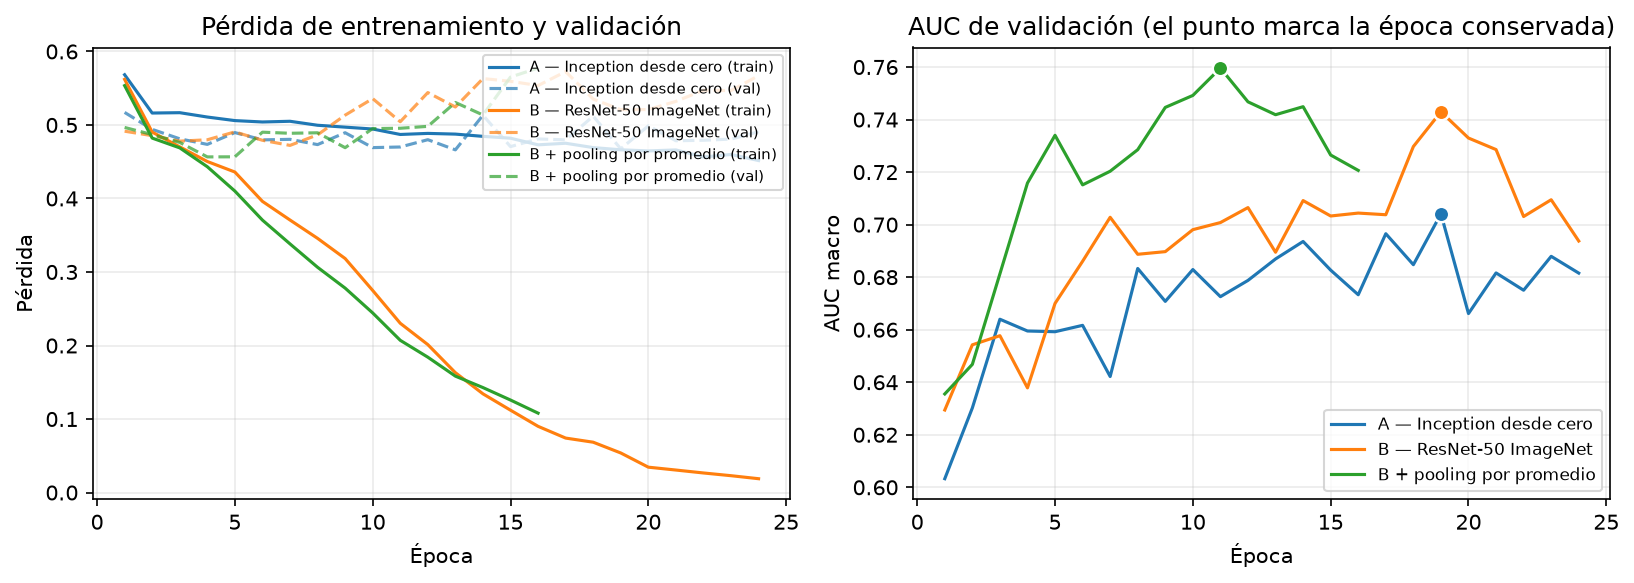
\includegraphics[width=0.60\textwidth]{figuras/curvas_entrenamiento.png}
\caption{Izquierda: pérdida de entrenamiento (línea continua) y de validación
         (discontinua). Derecha: AUC macro de validación; el punto marca la época
         que la detención temprana conserva.}
\label{fig:curvas}
\end{figure}

El sobreajuste es visible de inmediato. La razón entre la pérdida final de
validación y la de entrenamiento es de $5.7\times$ para ResNet-50 con promedio,
$3.2\times$ con atención y $1.1\times$ para Inception. Esta última mantiene ambas
curvas juntas por falta de capacidad, y obtiene el AUC más bajo de las tres.

\subsection{Comparación de las dos arquitecturas}

\begin{table}[ht]
\centering
\caption{Resultados sobre los estudios dorados. El umbral se selecciona en
validación y se aplica sin modificación. Los dos bloques son regímenes de datos
distintos y no se comparan entre sí; dentro de cada uno solo cambia la
arquitectura.}
\label{tab:principal}
\begin{tabular}{lrcccc}
\toprule
Configuración & Parám. & AUC macro & IC95\% & $F_1$ & Umbral \\
\midrule
\multicolumn{6}{l}{\emph{576 estudios, 8 grupos, una sola vista sagital}} \\
A --- Inception desde cero & 0.7~M & 0.628 & $[0.569, 0.687]$ & 0.484 & 0.25 \\
B --- ResNet-50 ImageNet & 24.1~M & 0.646 & $[0.579, 0.703]$ & 0.490 & 0.25 \\
B + agregación por promedio & 23.5~M & 0.708 & $[0.662, 0.755]$ & 0.560 & 0.20 \\
\midrule
\multicolumn{6}{l}{\emph{4\,407 estudios, 64 grupos, atención por etiqueta}} \\
C --- Inception, un modelo de 12 & 1.3~M & 0.638 & $[0.581, 0.693]$ & 0.500 & 0.15 \\
D --- Inception por caras & $3\times$1.3~M & 0.658 & $[0.607, 0.709]$ & 0.487 & 0.20 \\
E --- ResNet-50 por caras & $4\times$26.9~M & \textbf{0.761} & $[0.715, 0.810]$ & \textbf{0.588} & 0.20 \\
\bottomrule
\end{tabular}
\end{table}


La configuración E alcanza el mayor AUC macro puntual sobre los dorados, 0.761,
con $F_1$ de 0.588 al umbral 0.20 elegido en validación; su intervalo
$[0.715, 0.810]$ se solapa con el de ResNet-50 con promedio ($[0.662, 0.755]$),
de modo que el margen sobre este no es significativo. El análisis detallado
(desglose por etiqueta, Grad-CAM y sesgo) se hace sobre ResNet-50 con promedio y
no sobre E: E rutea cada etiqueta a un modelo distinto, de modo que no define un
único mapa de activación por estudio ni una matriz de confusión comparable entre
etiquetas. El umbral queda muy por debajo de 0.5, coherente con las prevalencias
bajas del Cuadro~\ref{tab:etiquetas}: un umbral de 0.5 descartaría casi todos los
positivos de las etiquetas raras.

Entre las dos arquitecturas del entregable \#2, ResNet-50 con ImageNet supera a
la Inception escrita desde cero por 0.018 de AUC, y el bootstrap pareado deja ese
margen dentro del ruido ($[-0.098, +0.058]$): con 56 estudios de prueba no se
puede afirmar. El segundo bloque cambia el veredicto, y el cambio proviene del
régimen y no de la arquitectura. Con 4\,407 estudios, ResNet-50 por caras supera
a Inception por caras en 0.103 con intervalos que no se solapan ($[0.715,
0.810]$ frente a $[0.607, 0.709]$), de modo que acá la diferencia sí se
sostiene. El empate del primer bloque describía un conjunto demasiado pequeño
para que el preentrenamiento rindiera, no una equivalencia entre los modelos.

\subsection{Desglose por etiqueta}

\begin{table}[ht]
\centering
\caption{Desglose por etiqueta sobre los estudios dorados. Las tres columnas de AUC corresponden a Inception (A), ResNet-50 (B) y ResNet-50 con promedio; el intervalo y la matriz de confusión son de esta última, al umbral 0.20 elegido en validación. Un asterisco marca los intervalos que incluyen 0.5: son 3 de 12, es decir hallazgos que no se distinguen del azar. La columna Prev.\ es la prevalencia de cada hallazgo sobre los 4\,349 estudios no dorados (distribución natural).}
\label{tab:etiquetas}
\begin{tabular}{lrrcccrrrrc}
\toprule
Etiqueta & Pos. & Prev. & A & B & Mejor (IC95\%) & TP & FP & FN & TN & $F_1$ \\
\midrule
Lig.\ cruzado ant. & 23 & 16.5\% & 0.714 & 0.706 & 0.776 $[0.64, 0.89]$ & 20 & 17 & 3 & 16 & 0.667 \\
Lig.\ colateral med. & 9 & 10.6\% & 0.496 & 0.520 & 0.638 $[0.44, 0.83]$$^{*}$ & 6 & 20 & 3 & 27 & 0.343 \\
Menisco medial & 24 & 45.5\% & 0.611 & 0.680 & 0.734 $[0.59, 0.86]$ & 22 & 18 & 2 & 14 & 0.687 \\
Menisco lateral & 23 & 26.0\% & 0.545 & 0.497 & 0.531 $[0.38, 0.69]$$^{*}$ & 16 & 18 & 7 & 15 & 0.561 \\
Osteoartrosis med. & 15 & 7.9\% & 0.680 & 0.720 & 0.816 $[0.68, 0.93]$ & 8 & 4 & 7 & 37 & 0.593 \\
Osteoartrosis lat. & 11 & 4.8\% & 0.610 & 0.655 & 0.693 $[0.51, 0.87]$ & 5 & 9 & 6 & 36 & 0.400 \\
Osteoartrosis PF & 20 & 26.3\% & 0.589 & 0.618 & 0.704 $[0.55, 0.84]$ & 19 & 31 & 1 & 5 & 0.543 \\
Derrame articular & 34 & 35.7\% & 0.749 & 0.729 & 0.619 $[0.46, 0.77]$$^{*}$ & 31 & 19 & 3 & 3 & 0.738 \\
Sinovitis & 25 & 10.1\% & 0.697 & 0.648 & 0.672 $[0.52, 0.81]$ & 17 & 16 & 8 & 15 & 0.586 \\
Quiste de Baker & 11 & 18.6\% & 0.648 & 0.640 & 0.731 $[0.51, 0.91]$ & 6 & 12 & 5 & 33 & 0.414 \\
Contusión ósea & 18 & 14.4\% & 0.594 & 0.652 & 0.773 $[0.64, 0.90]$ & 17 & 25 & 1 & 13 & 0.567 \\
Fractura & 17 & 7.6\% & 0.605 & 0.689 & 0.813 $[0.67, 0.93]$ & 13 & 12 & 4 & 27 & 0.619 \\
\bottomrule
\end{tabular}
\end{table}


Al umbral 0.20, el modelo del análisis detallado (ResNet-50 con promedio) alcanza
una precisión macro de 0.466 y un recall macro de 0.744; el $F_1$ macro, 0.560,
promedia ambas por etiqueta. El recall supera a la precisión porque el umbral bajo
prioriza no perder los positivos de las etiquetas raras.

Tres de las doce etiquetas no se distinguen del azar: su intervalo
incluye 0.5. El ancho medio del intervalo por etiqueta es 0.302 frente a 0.093
del macro: el macro es 3.3 veces más estrecho por aritmética, no por mayor
certeza. Los dos casos extremos fallan por razones distintas: el menisco
lateral tiene 23 positivos, suficientes, y aun así da 0.531 (el modelo no lo
detecta), mientras que el ligamento colateral medial tiene nueve y su intervalo
abarca 0.39 puntos, de modo que ni siquiera se puede decir si lo detecta.

\subsection{Reproducibilidad del entrenamiento}
\label{sec:reproducibilidad}

Dos entrenamientos de la misma configuración, con la misma semilla y los mismos
datos, divergían desde la primera época y llegaban a mejores AUC de 0.6501 y
0.6801; fijando los kernels, coinciden bit a bit (0.6633 y 0.6633). El origen no
fue un error de cálculo sino una suposición: que sembrar los generadores basta
para que un entrenamiento en GPU sea reproducible. No basta (cuDNN elige sus
kernels en tiempo de ejecución y varios acumulan en orden no determinista) y la
magnitud importa más que el hecho: la diferencia entre dos corridas idénticas
llegó a 0.041 de AUC macro, mayor que cuatro de las siete comparaciones que se
reportan más abajo. Mientras los kernels no estén fijados, ninguna distingue el
efecto buscado del ruido de ejecución, y el bootstrap no lo advierte: mide la
variabilidad del muestreo de estudios, no la de la ejecución.

Todos los resultados de este informe provienen de corridas con
\texttt{cudnn.deterministic}, \texttt{benchmark} desactivado,
\texttt{use\_deterministic\_algorithms} y \texttt{CUBLAS\_WORKSPACE\_CONFIG}
fijado antes de crear el contexto de CUDA. La verificación corre como una etapa
del pipeline y falla si las dos corridas no coinciden bit a bit, a un costo
despreciable (2.4 minutos contra 2.2 por corrida).

\paragraph{Reproducibilidad del pipeline.}
Todo el pipeline se ejecuta con un único comando,
\texttt{python pregunta1/paso6\_informe/ejecutar\_todo.py}, sobre las versiones
fijadas en \texttt{requirements.txt}; es idempotente y recompila el informe desde
los JSON versionados aun sin el dataset. El código, los pesos (\emph{release}
\texttt{v1.0-pesos}) y las pruebas unitarias en \texttt{tests/} están en el
repositorio: \url{https://github.com/sergiomc12/rnap-2026ii-p1-rodilla-mri}.

\subsection{Validación cruzada}
\label{sec:cruzada}

La validación cruzada sobre cinco pliegues da la escala con la que leer cualquier
diferencia medida sobre una sola partición: ResNet-50 con promedio alcanza
$0.7354 \pm 0.0125$ de AUC entre pliegues, con atención $0.6975 \pm 0.0143$ e
Inception con atención $0.6717 \pm 0.0150$. Con desviaciones de 0.014, una
diferencia menor a 0.03 sobre una sola partición no se distingue de la variación
entre pliegues (\texttt{paso3\_modelos/validacion\_cruzada.json}).

\subsection{Estudio de ablación}
\label{sec:ablacion}

\begin{table}[ht]
\centering
\caption{Bootstrap pareado sobre los estudios dorados. 2 de 7 diferencias alcanzan significancia, entendida como un intervalo del 95\% que no cruza cero. El bootstrap es \emph{pareado} —remuestrea los mismos estudios para las dos configuraciones— porque comparar dos intervalos independientes tiene mucha menos potencia.}
\label{tab:ablacion}
\begin{tabular}{lcccc}
\toprule
Comparación & $\Delta$ AUC & IC95\% & $P(A>B)$ & Signif. \\
\midrule
Inception vs.\ ResNet-50 & $-0.018$ & $[-0.098, +0.058]$ & 34\% & no \\
Promedio vs.\ atención & $+0.062$ & $[-0.001, +0.128]$ & 97\% & no \\
ImageNet vs.\ desde cero & $+0.084$ & $[+0.002, +0.165]$ & 98\% & \textbf{sí} \\
Focal vs.\ BCE (con atención) & $-0.025$ & $[-0.081, +0.034]$ & 20\% & no \\
Focal vs.\ BCE (con promedio) & $-0.016$ & $[-0.051, +0.016]$ & 16\% & no \\
BCE ponderada vs.\ BCE & $-0.009$ & $[-0.047, +0.027]$ & 31\% & no \\
Plano sagital vs.\ coronal & $+0.056$ & $[+0.005, +0.108]$ & 99\% & \textbf{sí} \\
\bottomrule
\end{tabular}
\end{table}


Solo dos de las siete comparaciones alcanzan significancia, y las dos
son sobre los datos, no sobre la arquitectura. El preentrenamiento en ImageNet
aporta $+0.084$ de AUC ($[+0.002, +0.165]$) y el plano sagital supera al coronal
en $+0.056$ ($[+0.005, +0.108]$, sobre los 54 estudios dorados que tienen ambos
planos). Ninguna de las cinco decisiones restantes (arquitectura, agregación,
función de pérdida en dos variantes y ponderación por clase) produce un efecto
que el intervalo distinga de cero.

\paragraph{La agregación por atención.} El promedio simple supera a la
agregación por atención en $+0.062$ de AUC, con el promedio preferido en el
97\% de los remuestreos, pero el intervalo roza el cero ($[-0.001, +0.128]$) y
por lo tanto la diferencia no se puede afirmar. La dirección es la esperable si
el módulo de atención sobreajusta (introduce parámetros entrenables sobre 416
estudios cuyas etiquetas tienen un 25.7\% de ruido, mientras que un promedio no
tiene parámetros y no puede sobreajustar), y es consistente en validación
(0.762 contra 0.724), pero afirmarla con 56 estudios de prueba sería ir más
lejos de lo que el dato permite.

\paragraph{Las decisiones sobre los datos sí pesan.} Las dos diferencias que
sobreviven al test son las que cambian \emph{qué ve} el modelo: de dónde vienen
sus pesos iniciales y qué plano se le muestra. Es coherente con lo que ocurre en
la extracción de etiquetas, donde la detección de negación y la traducción
produjeron los efectos de mayor magnitud de todo el trabajo: con 416 estudios de
entrenamiento y un 25.7\% de ruido en las etiquetas, lo que se le da al modelo
importa más que cómo está construido. En cambio, ninguna de las tres variantes de
pérdida evaluadas (focal con atención, focal con promedio, BCE ponderada)
mejora el resultado, y las tres tienen intervalos que cruzan cero.

\subsection{Interpretabilidad}

Se generaron mapas de activación para los tres hallazgos que pide el enunciado,
sobre ResNet-50 con promedio. En cada panel, de izquierda a derecha: el corte
original, el mapa de activación y la superposición de ambos.

\begin{figure}[htbp]
\centering
% Las tres son paneles de relacion 3:1, asi que apiladas ocupan alto en
% proporcion a su ancho. Bajaron a 0.35 para que el cuerpo entre en las 10
% paginas que pide el enunciado tras incorporar la columna de prevalencia y las
% metricas de precision/recall: los paneles se siguen leyendo.
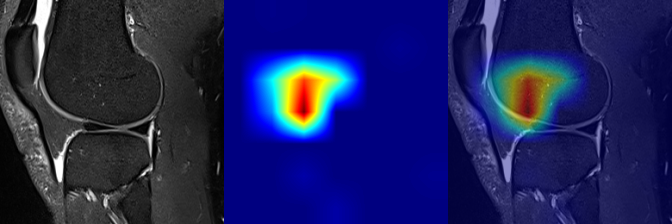
\includegraphics[width=0.30\textwidth]{figuras/gradcam_Effusion.png}
\vspace{1pt}
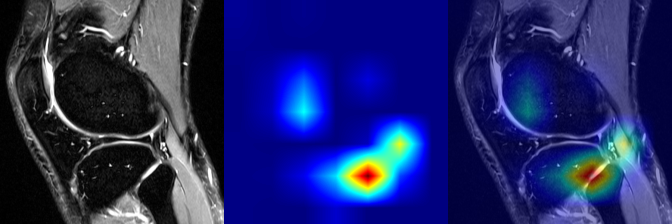
\includegraphics[width=0.30\textwidth]{figuras/gradcam_ACL.png}
\vspace{1pt}
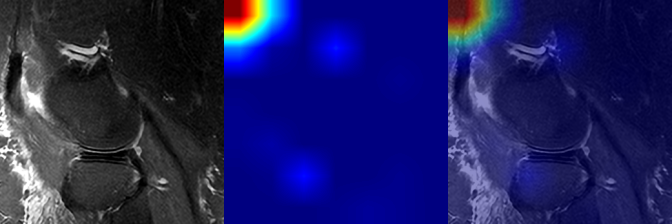
\includegraphics[width=0.30\textwidth]{figuras/gradcam_Medial_Meniscus.png}
\caption{Grad-CAM sobre ResNet-50 con promedio.
         \emph{Arriba}, derrame articular ($p = 0.576$): la activación se
         concentra en el receso suprapatelar, donde el líquido se acumula.
         \emph{Centro}, ligamento cruzado anterior ($p = 0.815$): cubre la
         región intercondílea, donde el ligamento se inserta. \emph{Abajo},
         menisco medial ($p = 0.406$): la activación cae fuera de la
         articulación. Es el caso menos plausible anatómicamente: la predicción
         es correcta, pero la activación cae fuera de la articulación.}
\label{fig:gradcam}
\end{figure}

Los dos casos plausibles son los de mayor probabilidad predicha. El menisco
medial es el más informativo: con $p = 0.406$ el modelo lo predice correctamente
y su AUC de 0.734 está entre los mejores, pero Grad-CAM muestra que esa predicción
se apoya en una región fuera de la articulación.

Para distinguir un patrón de una coincidencia, el procedimiento se repitió sobre
ocho estudios dorados positivos de cada uno de los doce hallazgos, midiendo el
centro de masa de la región activada en coordenadas normalizadas.

Solo 3 de los doce hallazgos tienen activación consistente
(dispersión del centro de masa menor a 0.20 y ningún caso en el margen,
medido en \texttt{paso5\_ablacion\_gradcam/patron\_gradcam.json}); el derrame
articular y el ligamento cruzado anterior están entre ellos, y la medición
coincide con la figura. En los nueve restantes la evidencia varía demasiado entre
casos como para considerarla anatómicamente localizada. Dado que el
preprocesamiento recorta 130\,mm centrados en la rodilla, una activación en el
margen no puede corresponder a la articulación.

Esto tiene lectura clínica directa: las predicciones dudosas se apoyan en
regiones que no corresponden a la anatomía del hallazgo y, como los umbrales
caen entre 0.10 y 0.30, se convierten en positivos.

\subsection{Desbalance de clases}

La columna Prev.\ del Cuadro~\ref{tab:etiquetas} da la prevalencia de cada uno de
los doce hallazgos sobre los 4\,349 estudios no dorados: va del 4.8\%
(osteoartrosis del compartimento lateral) al 45.5\% (daño de menisco medial), un
factor de 9.5 entre extremos. El muestreo por cuotas descrito en la metodología
reduce ese factor a unos 4.5 en el subconjunto de 576 estudios con que se
entrenan las configuraciones A--B, mitigando en parte el desbalance.

Se evaluaron dos mitigaciones. La entropía cruzada binaria ponderada asigna a
cada etiqueta un peso inversamente proporcional a su prevalencia, con tope en 10
para que una etiqueta casi ausente no desestabilice el entrenamiento. La pérdida
focal~\citep{lin2017focal} reduce la contribución de los ejemplos ya resueltos:
con $\gamma=2$ y $\alpha=0.25$ disminuye 880 veces el aporte de un ejemplo fácil
y solo 2.2 veces el de uno difícil.

Ninguna de las dos mejora el AUC macro, y ninguna lo empeora de forma que el test
distinga: la ponderada da $\Delta = -0.009$ (IC95\%
$[-0.047, +0.027]$) y la focal
$\Delta = -0.016$ (IC95\% $[-0.051, +0.016]$).
Por etiqueta rara el resultado se reparte sin patrón, y con 56 estudios esas
diferencias están dentro del ruido. El desbalance no es la restricción dominante
de este problema; el 25.7\% de ruido en las etiquetas de entrenamiento sí lo es.

% ============================================================================
\section{Sesgo geográfico y lingüístico}
% ============================================================================

La calidad de la extracción de etiquetas varía de forma pronunciada entre
idiomas. Antes de la traducción, el $F_1$ macro iba de 0.66 en inglés a 0.00 en
croata, griego y búlgaro: el pipeline producía supervisión utilizable para el
55\% de los estudios y ruido para el 45\% restante, en correlación directa con el
país del centro emisor.

La traducción mitiga el problema sin eliminarlo. El griego permanece con un
54.2\% de estudios sin ninguna etiqueta, frente al 11.5\% del inglés. La
degradación terminológica del traductor es observable de forma directa:
\emph{knee} traducido como \emph{eye}, \emph{cruciate} como \emph{cross-linked},
y lo que presumiblemente era \emph{effusion} como \emph{urinary growth}.

Un modelo entrenado sobre estas etiquetas aprende predominantemente de estudios
redactados en inglés o español. Desplegado en un centro que informa en griego o
búlgaro, su rendimiento real sería inferior al reportado y ninguna métrica
agregada lo advertiría: un AUC macro de 0.708 no transparenta que la supervisión
fue sistemáticamente peor para unos centros que para otros. El sesgo está en los
datos que lo alimentan, no en el modelo, y es invisible a una auditoría que
examine solo las predicciones.

Existe además un límite no verificable: de los 4\,349 estudios sin etiqueta
dorada, 1\,989 corresponden a los siete idiomas problemáticos y su calidad de
etiqueta no admite medición, porque no hay verdad de referencia para ellos. Lo
que este informe reporta se estima sobre los 30 estudios dorados no ingleses y se
extrapola bajo el supuesto, no verificable, de que el extractor se comporta
igual. La consecuencia práctica es que la validación local sería indispensable
antes de operar en un centro cuyo idioma no estuviera bien representado.

% ============================================================================
\section{Discusión crítica de las limitaciones}
% ============================================================================

\paragraph{Tamaño de muestra.}
Los 56 estudios dorados producen un intervalo del 95\% de aproximadamente
$\pm0.05$ sobre el AUC macro, y de 0.30 en promedio por etiqueta individual; cada
pliegue de la validación cruzada emplea 104 estudios con etiqueta débil. Eso fija
el tamaño mínimo de efecto que este trabajo puede detectar, y explica por qué
cinco de las siete comparaciones de la ablación quedan sin resolver.

\paragraph{El 25.7\% de etiquetas incorrectas es un techo, y parte de él es irreducible.}
Parte de ese ruido no se puede eliminar desde el texto: un informe que consigna
\emph{Moderate joint effusion} tiene la etiqueta de derrame en cero, y otro que
menciona \emph{osteochondral fracture} tiene la de fractura en cero, porque media
criterio clínico: una fractura osteocondral en la faceta rotuliana se
contabiliza como osteoartrosis patelofemoral. Sinovitis es el caso extremo: 8 de sus 17 positivos
perdidos no mencionan nada sinovial en todo el informe, de modo que ampliar el
léxico no la recupera. Queda sin evaluar como factor de ablación ponderar por
confianza frente a entrenar solo con estudios de alta confianza, la comparación
más pertinente dado que el ruido de etiqueta domina el resultado.

\paragraph{Sobre la agregación por atención no se puede concluir nada.}
Queda por detrás del promedio simple en los dos conjuntos, pero el intervalo de
la diferencia cruza cero: con 56 estudios de prueba su aporte no es medible.

\paragraph{La activación es consistente en solo tres de doce hallazgos.}
Medido sobre ocho estudios por hallazgo, la dispersión del centro de masa se
mantiene por debajo de 0.20 sin ningún caso en el margen únicamente para el
ligamento cruzado anterior, el menisco lateral y el derrame articular. En los
nueve restantes la evidencia en que el modelo se apoya varía demasiado entre
casos como para considerarla anatómicamente localizada, y todos presentan algún
caso cuya activación cae en el borde de la imagen, fuera de la articulación. El
menisco lateral figura entre los tres pese a un AUC de 0.531
(Cuadro~\ref{tab:etiquetas}): la activación consistente no implica una predicción
correcta.

\section{Conclusiones}
% ============================================================================

Los resultados principales son tres.

Primero, casi ninguna intervención del lado del modelo fue
significativa: de las siete de la ablación, solo el preentrenamiento en ImageNet
($+0.084$) y el plano de la resonancia ($+0.056$).

Segundo, eso describe el régimen y no las arquitecturas: con 4\,407
estudios en lugar de 576, ResNet-50 supera a Inception por 0.103 de AUC con
intervalos que no se solapan. El empate del entregable \#2 medía un conjunto
demasiado pequeño para que el preentrenamiento rindiera. Por eso la comparación debe
declarar el régimen de datos.

Tercero, un entrenamiento en GPU no es reproducible por sembrar los
generadores: dos corridas con la misma semilla llegaban a diferir 0.041 de AUC,
por encima de cuatro de las siete comparaciones del estudio. Con los kernels
fijados, el efecto de la atención frente al promedio queda en $[-0.001, +0.128]$
y no alcanza significancia; el bootstrap, que mide el muestreo de estudios y no la
ejecución, no advertía esa variabilidad.

La limitación de fondo persiste: 56 estudios no distinguen efectos menores a
0.05 de AUC. En la configuración E, de mayor AUC macro, sinovitis (0.559) y
artrosis patelofemoral (0.592) quedan cerca del azar sobre los dorados, lo que
sugiere que para esas dos etiquetas el modelo predice al extractor y no al
hallazgo.

\bibliographystyle{plainnat}
\bibliography{referencias}

\end{document}
